% Este archivo es parte de la memoria del proyecto fin de carrera
% de Manuel López Urbina. Protegida bajo la licencia GFDL.
% Para más información, la licencia completa viene incluida en el
% fichero fdl-1.3.tex

% Copyright (C) 2018 Manuel López Urbina

\newpage

\chapter[Requisitos]{Especificación y análisis de requisitos}
\label{chap:requisitos}

En el presente capítulo se recopilan las diferentes carcaterísticas base de obligado cumplimiento por el producto final a desarrollar. Siendo estas características definidas en una
etapa incial del presente proyecto. \\

Debido a que el proyecto implica un desarrollo tanto a nivel software como hardware se realizó una recopilación de requisitos abarcando ambas áreas por separado.\\

\section{Requerimientos hardware}
\label{sec:requerimientos-hardware}

Se ha optado por la construcción de un robot móvil dotado de un chasis de 4 ruedas donde las dos ruedas traseras serán accionadas por un motor mientras que las dos ruedas delanteras
harán de directrices.\\

El motor porpulsor funcionará a corriente continua de manera que en función de la polarización de los terminales haga girar las ruedas en una dirección o la contraria (marcha adelante o atrás), mientras que 
la dirección será accionada por un servomotor.\\

El chasis utilizado deberá permitir añadir multitud de componentes necesarios para construir el robot, deberá disponer de paneles para instalar las diferentes
placas electrónicas y sensores además de ser lo suficientemente liguero para que el sistema en su conjunto tenga agilidad en sus movimientos a la vez que resistencia.\\

El robot además deberá poder obtener imágenes de vídeo y transmitirlas al servidor donde se encuentre alojada la aplicación de control. Por lo que resulta necesario incorporar una cámara de 
pequeñas dimensiones de alta definición.\\

Por otra parte, todo robot necesita de una unidad de central de procesamiento donde se localizará el programa de control. Este programa tendrá la función de interpretar las diferentes señales recibidas,
control de sensores y dispositivos conectados. Además, esta placa es la encargada de distribuir la alimentación por los diferentes componentes hardware que lo necesiten y recibir las señales de
los sensores y enviarla a los motores.\\

Necesidad de poder acoplar multitud de sensores para medicíon de parámetros ambientales resultando necesario incorporar alguna placa dotada de un microcontrolador de fácil programación como podría ser
algunas de las placas proporcionadas por Arduino.\\

Tanto la placa que incorpore el microcontrolador y sus sensores como la unidad central de procesamiento deben disponer de un canal de comunicación para el intercambio de datos entre las mismas.\\


\subsection{Análisis y selección de componentes electŕonicos}

La informática, en los últimos años ha dado un gran impulso con proyectos como el de la Raspberry Pi Foundation, en este caso concreto en áreas como la del IOT \footnote{
Internet de las cosas (en inglés, Internet of Things, abreviado IoT o​ IdC, por sus siglas en español​) es un concepto que se refiere a la interconexión digital de objetos cotidianos
con Internet.​}. En lo referente al hardware, nunca ha sido más fácil coger componentes, juntarlos y con una mínima programación hacer algo totalmente nuevo, interesante y útil al
mismo tiempo gracias a la existencia de proyectos como Arduino.\\

En este caso, nos planteamos la siguiente incógnita; ¿Empleamos una Raspberry Pi o un Arduino?. En internet encontramos tantos y tantos proyectos por 
hacer en los que muchas veces es difícil decidirse.\\

Arduino se compone de una parte Hardware y Software. Es por ello que gracias a los emuladores existentes y sin tocar una sola pieza hardware, podemos simular un proyecto desde 
nuestro ordenador. Podemos programarlo y hacer las conexiones virtuales para ver cómo se comportaría. Arduino es una plataforma simple y dedicada precisamente a eso, 
a montar sobre ella los componentes necesarios para los proyectos. \\

La Raspberry Pi Foundation en cambio, ha diseñado y elaborado un ordenador para enseñar informática a la antigua usanza. La Raspberry Pi es un ordenador asequible, 
suficientemente potente para facilitar el aprendizaje y realizar tareas básicas. Incluso programar y compilar programas que se ejecuten en la Raspberry Pi. Y todo ello en un
tamaño mínimo, similar al de una tarjeta de crédito, alimentado con un cargador de móvil de 2 amperios y que da muchísimo juego para todo tipo de proyectos.\\

Por tanto, en respuesta a la pregunta inicial, se ha decidido que la mejor placa la elaboración del proyecto es aprovechar lo mejor de cada una de ellas. Utilizaremos tanto una Raspberry Pi
como una Arduino Mega aprovechando al máximo el potencial que ofrece cada una de ellas, cada una con sus virtudes y sus defectos.\\


\subsubsection{Ventajas y desventajas de Raspberry Pi y de Arduino}


%REFERENCIA https://www.xataka.com/makers/raspberry-pi-frente-a-arduino-quien-se-adapta-mejor-a-mi-proyecto-maker

Sabemos que Arduino no destaca precisamente por su potencia de cálculo, ni la memoria de la placa, ni la frecuencia del procesador. Entonces, ¿Por qué Arduino es masivamente utilizado
en multitud de proyectos? Arduino destaca por su la facilidad de conectarse con el mundo, gracias a las entradas tanto analógicas como digitales con las que
cuenta y de lo fácil que resulta activar o desactivar una de las entradas/salidas gracias a su software.

La placa Arduino Mega empleada en el presente trabajo dispone 54 pines de entrada salida digital, de los cuales quince de ellos pueden ser utilizados como salidas PWM y controlar 
con ellos la velocidad de motores, lectura de sensores, activación de servomotores, por citar algunos de los múltiples ejemplos y posibilidades. También tiene 16 entradas analógicas, una frecuencia de 16 MHz y un conector USB y un ICSP y 4 UART. Existen muchísimos tipos de
placas Arduino y cada una con sus características específicas.\\

Otro punto a favor su la facilidad de prototipado donde los Shields o placas de expansión, ofrecen a nuestra placa funcionalidades añadidas que van desde conectividad Wi-Fi, 
GPS, conectividad por radio, pantallas, displays táctiles, etc. Y muchas de ellas con un bajo coste.\\

Por el contrario la Raspberry Pi puede presumir de una potencia de cálculo muco más elevada comparada con las placas Arduino. Posee además mayor cantidad de memoria y capacidades
multimedia, que van desde la reproducción de video en HD, pasando por una salida de audio, así como una salida HDMI. Esto hacen que pese a no contar con las capacidades de
interconexión de Arduino, sí que existan placas de expansión en forma de shields. Posible gracias a los conectores GPIO, I2S, etc. que incorpora la Raspberry Pi.\\

\begin{figure}[H]
  \begin{center}
    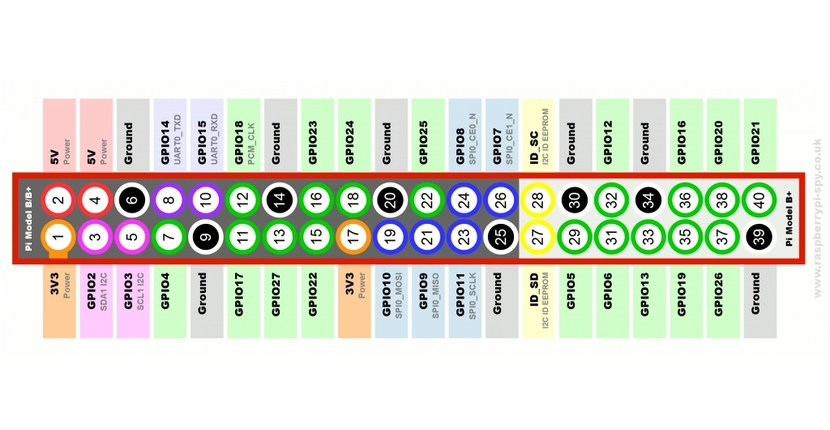
\includegraphics[scale=0.4]{imagenes/robot/gpio-conexiones.jpg}
  \end{center}
  \caption{Esquema GPIO de una Raspberry Pi Model B+.}
  \label{gantt:tareas01}
\end{figure}

Por otra parte, otro de los puntos a tener muy en cuenta es la posibilidad de incorporar las diferentes cámaras desarrolladas de diversas características y tipos diferentes como
la captación de imágenes por infrarrojos, nos damos cuenta de que la Raspberry Pi puede sustituir a un ordenador en tareas simples. Y además podemos usar sus puertos de conexión
para interconectar nuestro proyecto con el mundo como lo haríamos con un Arduino.\\

\begin{figure}[H]
  \begin{center}
    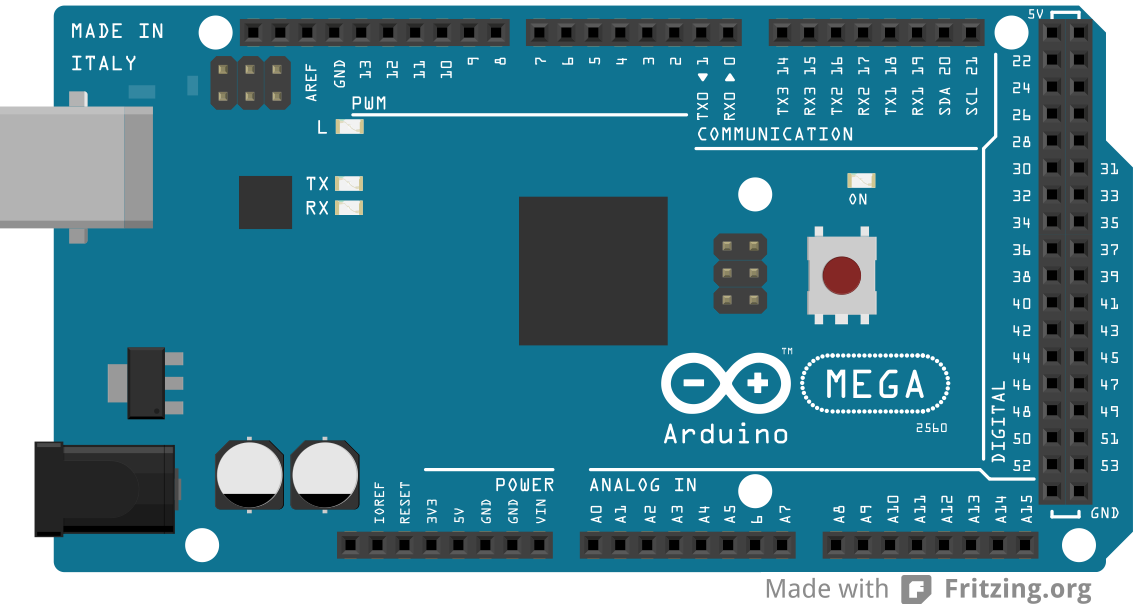
\includegraphics[scale=0.4]{imagenes/arduino_mega_pinout.png}
  \end{center}
  \caption{Placa Arduino Mega donde se visualiza la disposición de sus pines E/S.}
  \label{gantt:tareas01}
\end{figure}

Por tanto, de todo lo anterior podemos concluir Arduino y Raspberry Pi son herramientas complementarias y perfectamente utilizables para cumplir con los requisitos del presente proyecto.\\\\


\section{Requerimientos software}
\label{sec:requerimientos-software}

Habiendo detallado los requerimientos hardware para la construcción del robot pasamos al análisis de los diferentes requerimientos software para la correcta
gestión de los diferentes elementos hardware utilizados y para su correcto funcionamiento.\\

En cuanto a la programación del robot, uno de los requisitos fundamentales es el de disponer de una vía de comunicación bidireccional junto con la posibilidad de
configurar una interfaz de control personalizada en función de los sensores que se deseen utilizar y según las características del medio al que queramos adaptar nuestro vehículo.\\

Otro requerimiento software es el de la posibilidad de integrar la lectura de valores obtenidos por sensores mostrando al usuario los parámetros obtenidos y envío de órdenes
desde un servidor externo. Además de captación y transmisión de vídeo en tiempo real.\\

Todas estas especificaciones quedan resueltas mediante la utilización de la aplicación web RobotUI, la cual se ha decidido utilizar como parte software del presente proyecto.\\

Para el caso que nos concierne en el proyecto, dentro del marco de investigación que define la totalidad de la infraestructura, la funcionalidad principal del mismo a nivel 
software será:\\

\begin{itemize}
\item Definir los pasos para dar de alta un dispositivo robótico en el sistema.
\item Una vez configurado el dispositivo, configurar la interfaz de control con las acciones de control específicas.
\item Realizar un sistema de monitorización y visualización para los usuarios espectadores en tiempo real.
\item Sistema de gestión de base de datos en donde se encuentren los datos de la aplicación recogidos.
\item Panel de administración donde visualizar la información de los usuarios conectados y dispositivos en uso en tiempo real.
\end{itemize}

\section[Especificación]{Especificación de los requisitos}

En esta etapa del modelado de requisitos se captura el propósito general del sistema:

\begin{itemize}
\item Se analiza qué debe hacer el sistema.
\item Se obtiene una versión contextualizada del sistema.
\item Identifica y delimita el sistema.
\item Se determinan las características, cualidades y restricciones que debe satisfacer el sistema.
\end{itemize}

\subsection{Requisitos funcionales}

Los requisitos funcionales que se han obtenido en el sistema son los siguientes:

\begin{itemize}
\item Ser una herramienta multiplataforma y que permita a cualquier usuario definir sus propias interfaces para el control de robots.
\item Dotar de funcionalidad gráfica que permita en tiempo real con mecanismos visuales (en web) visualizar el control de dispositivos robóticos por parte de otros usuarios, modo espectador de la aplicación.
\item Proporcionar un sistema de streaming de vídeo para la difusión de imágenes a los usuarios espectadores procedentes de los robots dispongan de cámara.
\item Implementar un panel de administración para la visualización de usuarios y dispositivos conectados en tiempo real.
\end{itemize}

\subsection{Requisitos no funcionales}

Los requisitos no funcionales son aquellos que describen cualidades o restricciones del sistema que no se relacionan de forma directa con el comportamiento funcional del mismo. A continuación se especifican los más importantes del sistema:
\begin{itemize}
\item No requiere un conocimiento específico del sistema una vez puesto en funcionamiento.
\item La aplicación tendrá manual de uso.
\item La base de datos estará implementada en un lenguaje objeto no relacional como MongoDB.
\item La aplicación estará realizada en el lenguaje de programación Python.
\item La interfaz debe reflejar claramente la distinción entre las distintas partes del sistema.
\item El sistema se desplegará sobre una versión GNU Linux Debian 8 Jessie.
\item El código fuente de la aplicación seguirá un estilo uniforme y normalizado para todos los módulos del mismo.
\end{itemize}
